% Template for taking notes\writing down exercise solutions
% In the specific context of mathematical Curricular Units

% In order to draw Finite State Machines\Turing Machines,
% we make use of the tikz-automata library
\documentclass[compress,svgnames,handout,13.7pt]{beamer}
\mode<presentation>
\usepackage[portuguese]{babel}
\usepackage{tikz}
\usetikzlibrary{automata, positioning, arrows}
\usepackage{makeidx,verbatim}
\usepackage{latexsym,amsfonts,amsmath,amssymb,amsthm}
\usepackage{curves}
\usepackage{enumerate}
\usepackage{moreverb}
\usepackage{cases}
\usepackage{array}
\usepackage{verbatim}
\usepackage{epsfig}
\usepackage{graphics}
\usepackage{float}
\usepackage{color}
%%\usepackage[latin1]{inputenc}
\usepackage{stmaryrd}
\usepackage{amstext}
\usepackage{xspace}
\usepackage[mathcal]{euscript}
\usepackage{rotating}
\usepackage{mathrsfs}
\usepackage{pgf,pgfnodes,pgfheaps}
\usepackage{listings}
\usepackage{xcolor}
\usepackage{listings}
\usetikzlibrary{arrows,automata,backgrounds}

\usecolortheme{seahorse}
\usecolortheme{rose}
\usefonttheme[onlylarge]{structuresmallcapsserif}
\setbeamerfont{frametitle}{family=\rmfamily,size=\footnotesize}
\setbeamercolor{title}{fg=blue!80!black}%,bg=blue!20!white}
\setbeamercolor{frametitle}{fg=blue!80!black}%,bg=blue!20!white}
\setbeamercolor{institute}{fg=blue!80!black}
\setbeamertemplate{miniframes}[tick]
\setbeamercovered{still covered={\opaqueness<1->{4}},
	again covered={\opaqueness<1->{4}}}
\setbeamerfont{small}{size=\small} \setbeamerfont{tiny}{size=\tiny}
\setbeamercolor{caixa}{fg=black,bg=blue!10!white}
\setbeamertemplate{navigation symbols}{}
\addtobeamertemplate{footline}
    {\leavevmode%
    \hbox{%
    \begin{beamercolorbox}
        [
        wd=\paperwidth,
        ht=2.75ex,
        dp=.5ex,
        right,
        rightskip=1em
        ]
        {mycolor}%
    \usebeamercolor[fg]{navigation symbols}
    \insertslidenavigationsymbol%
    \insertframenavigationsymbol%
    \insertsubsectionnavigationsymbol%
    \insertsectionnavigationsymbol%
    \insertdocnavigationsymbol%
    \insertbackfindforwardnavigationsymbol%
    \end{beamercolorbox}%
    }%
    \vskip0.5pt
 }{}

\def\N{{\mathbb N}}
\newcommand{\Z}{\mathbb Z}
\newcommand{\R}{\mathbb R}
\newcommand{\Q}{\mathbb Q}
\def\dotminus{\mathbin{\ooalign{\hss\raise1ex\hbox{.}\hss\cr\mathsurround=0pt$-$}}}
\def\proof{\noindent{\bf\blue Proof}\ }
			
\def\red{\color[rgb]{0.8,0,0}}
\def\lightred{\color[rgb]{1,0.5,0.5}}
\def\green{\color[rgb]{0,0.5,0}}
\def\lightgreen{\color[rgb]{0.5,1,0.5}}
\def\blue{\color[rgb]{0,0,0.7}}
\def\darkredblue{\color[rgb]{0.4,0,0.4}}
\def\lightgray{\color[rgb]{0.7,0.7,0.7}}
\def\mystep#1#2{\uncover<#1->{{\color<#1>[rgb]{0,0,1}{#2}}}}
\definecolor{azul}{rgb}{0,0,.7}
\definecolor{codegreen}{rgb}{0,0.6,0}
\definecolor{codegray}{rgb}{0.5,0.5,0.5}
\definecolor{codepurple}{rgb}{0.58,0,0.82}
\definecolor{backcolour}{rgb}{0.95,0.95,0.92}
\tikzset{->,
    >=stealth',
    node distance=3cm,
    every state/.style={thick, fill=gray!10},
    initial text=$ $,
}

\lstdefinestyle{mystyle}{backgroundcolor=\color{backcolour},
    commentstyle=\color{codegreen},
    keywordstyle=\color{magenta},
    numberstyle=\tiny\color{codegray},
    stringstyle=\color{codepurple},
    basicstyle=\ttfamily\footnotesize,
    breakatwhitespace=false,
    breaklines=true,
    captionpos=b,
    keepspaces=true,
    numbers=left,
    numbersep=5pt,
    showspaces=false,
    showstringspaces=false,
    showtabs=false,
    tabsize=2
}


\renewcommand\qedsymbol{QED}

\newcommand{\mycomment}[1]{}

\title[Apresentação Final]
    {\textbf{Mademoiselle Borges: Um Sistema de Bases de Dados para
Gestão de Eventos em Eventopolis\\
    \textbf{Grupo 06} \\
    \textit{Bases de Dados}}
}

\author[G06]{%
  \begin{tabular}{c}
    Bruno Gião \\
    A96544
  \end{tabular}
  \begin{tabular}{c}
    João Pereira \\
    A95375
  \end{tabular}
  \begin{tabular}{c}
    Helena Salazar \\
    A75635
  \end{tabular}
  \begin{tabular}{c}
    Tiago Teixeira \\
    A97666
  \end{tabular}
}


\date{\today}




\usetheme{CambridgeUS}
%\setbeamercovered{transparent}
\setbeamercovered{invisible}
\begin{document}


% Title Page
\thispagestyle{empty}
\frame{\titlepage}


% Table of Contents
\begin{frame}{Conteúdo}
\setcounter{secnumdepth}{2}
\setcounter{tocdepth}{2}
\tableofcontents
\end{frame}


\section{Introdução}

\subsection{Apresentação do Caso de Estudo}
\begin{frame}{Apresentação do Caso de Estudo}
Este trabalho consistirá na elaboração de um SBD que consiga, aptamente, ajudar Henrique Borges
e a c\^amara municipal de Eventopolis a gerir e publicitar os seus eventos.
\end{frame}

\section{Metodologia}

\subsection{Definição do Sistema}

\subsubsection{Contextualização}
\begin{frame}{Contextualização}
Em Eventopolis, uma localidade remota no centro de uma densa floresta, a gestão dos eventos sempre foi baseada em \textit{outsourcing} ou métodos manuais, devido à escassez de recursos humanos e à exist\^{e}ncia de um monopólio na área de Bases de Dados (BD). Este monopólio era controlado por uma seita de ocultistas tecnológicos, os quais praticavam preços exorbitantes e limitavam o acesso a uma parte significativa das informações nas suas bases de dados. Após uma revolta motivada pela insatisfação com a direção da empresa, alguns ex-membros, descontentes com a situação, optaram por adotar uma abordagem mais humanista e criar uma \textit{start-up} de Engenharia de Software em Eventopolis.
    
    Ao tomar conhecimento desta informação, o Professor Doutor Henrique Borges, responsável atual pela Gestão de Eventos na Câmara Municipal da cidade, prontamente identificou a oportunidade de mitigar os prejuízos significativos dos últimos anos ao estabelecer um contrato com a referida \textit{start-up} para a implementação de um sistema de Bases de Dados \textit{open-source}.
\end{frame}
\begin{frame}{Contextualização}
 O sistema de Bases de Dados seria batizado de ``Mademoiselle Borges'' em homenagem a Antoinette Borges, a antiga gestora de Eventos da Câmara Municipal de Eventopolis e esposa de Henrique Borges, que faleceu há alguns anos. Antoinette enfrentou uma pressão considerável ao depender da seita ou ao ser forçada a gerir manualmente os eventos com uma equipa de funcionários bastante limitada, desafios que foram fatores cruciais para o seu falecimento precoce.
   
Para Henrique Borges, este projeto tem então um significado profundamente pessoal. Além de simplificar o funcionamento dos eventos, diminuindo a mortalidade deste posto de trabalho, a criação deste Sistema também reflete a sua vontade de fomentar a promoção da arte e da cultura na sua pequena cidade, algo que era o maior sonho da sua falecida esposa. Antoinette queria ver a transformação da modesta e isolada cidade numa capital cultural, uma aspiração que, infelizmente, apenas se concretizaria após o seu falecimento.
\end{frame}
\begin{frame}{Contextualização}
Durante todos os eventos aprovados pela Câmara a cidade será transformada num cenário requintado que exalta a estética do estilo \textit{Art Nouveau}, o estilo artístico predileto da \textit{Mademoiselle}, este estilo tira inspiração da vegetação exuberante, densa e colorida, característica das imensas florestas que rodeiam Eventopolis. O principal local de eventos será uma gigantesca estufa situada no parque central, construída no início do século anterior. Esta estrutura possui uma cúpula central e vitrais coloridos, com um esqueleto de ferro com linhas detalhadas e artísticas, que ao longo do tempo oxidaram e agora exibem uma tonalidade verde clássica.
\end{frame}

\subsubsection{Fundamentação}
\begin{frame}{Fundamentação}
Considerando o modo prévio de gerir eventos em Eventopolis, onde o uso de serviços externos era considerado excessivamente dispendioso, e diante da escassez de recursos humanos para uma gestão manual, a única alternativa viável, na perspetiva de Henrique Borges, seria desenvolver um SBD interno.
\end{frame}

\subsubsection{Objetivos}
\begin{frame}{Objetivos}
    O Professor Doutor Henrique Borges acredita que a introdu\c{c}\~{a}o de uma base de dados
    trar\'{a} sucesso aos eventos.

    Os objetivos mencionados abaixo s\~{a}o fundamentais para refletir este sucesso:
    \begin{itemize}
    \item Aumentar a capacidade de armazenamento de informa\c{c}\~{o}es;
    \item Saber em tempo real qual a previsão de afluência de cada evento, sendo assim possível
planear os eventos com maior precisão;
    \item Perceber quais são os colaboradores com melhor desempenho nas vendas, permitindo o
uso de incentivos para estimulá-los a alcançar novos patamares de vendas;
    \item Possibilitar uma gestão financeira mais abrangente e precisa;
    \item Garantir que é minimizada a possibilidade da capacidade do evento ser excedida;
    \end{itemize}
\end{frame}
\begin{frame}{Objetivos}
    \begin{itemize}
        \item Obter, em tempo real, um registo preciso das compras de cada participante, bem como
identificar os itens mais vendidos tanto em eventos específicos quanto globalmente;
        \item Melhorar a organiza\c{c}\~{a}o de hor\'{a}rios para cada evento;
        \item Promover a cidade no \^{a}mbito nacional e internacional;
        \item Estimular a economia local por meio de inje\c{c}\~{a}o de capital na regi\~{a}o;
    \end{itemize}
\end{frame}

\subsubsection{Viabilidade}
\begin{frame}{Viabilidade}
O Professor Doutor Henrique Borges defende que ao implementar um sistema de controlo de eventos
        será possível: 
        \begin{itemize}
          \item Recuperar, no final no primeiro semestre, $40\%$ das perdas anteriores e cerca de $20\%$
            do investimento inicial;
          \item Aumentar a participação nos eventos em $20\%$;
        \end{itemize}
\end{frame}

\subsubsection{Recursos a Utilizar}
\begin{frame}{Recursos a Utilizar}
Recursos Humanos:
\begin{itemize}
               \item Pessoal de limpeza;
               \item Equipa de seguran\c{c}a;
               \item Vendedores;
               \item Equipa de multim\'edia;
               \item Funcion\'{a}rios da empresa de desenvolvimento;
               \item Potenciais Volunt\'arios.
             \end{itemize}
Recursos Materiais:
\begin{itemize}
             \item{Hardware:}
               \begin{itemize}
                 \item 1 servidor fornecido pela \textit{start-up} com 128GiB;
                 \item 15 terminais ``burros'';
                 \item 10 computadores pessoais.
               \end{itemize}
             \item{Software:}
               \begin{itemize}
                 \item SGBD;
                 \item Aplicação de vendas e aprovisionamento;
                 \item Redes sociais para divulgar o calendários dos eventos.
               \end{itemize}
             \end{itemize}
\end{frame}

\subsubsection{Equipa de Trabalho}
\begin{frame}{Equipa de Trabalho}
\begin{itemize} 
                 \item{\textbf{Pessoal Interno}}
                   Na equipa de gest\~ao de eventos da C\^amara Municipal de Eventopolis temos:
                   \begin{itemize}
                     \item{Professor Doutor Henrique Borges:} O coordenador principal da equipa;
                     \item{Maria Ivanovna Ivanova:} Colaboradora com experi\^encia em \textit{marketing} e co-coordenadora
                       da equipa;
                     \item{Herr Otto Mustermann:} Trabalhador \textit{part-time}.
                   \end{itemize}
                 \item{\textbf{Pessoal Externo}}
                   Já o pessoal externo, consiste na equipa de desenvolvimento da ``start-up'',
                   que seria constituída por 4 engenheiros, nomeadamente:
                   \begin{itemize}
                     \item Luke Bytespell
                     \item Aurelius Cibern\'etico
                     \item Bella Firewall
                     \item Aurora Matrix
                   \end{itemize}
             \end{itemize}
\end{frame}

\subsubsection{Plano de Execução do Trabalho}
\begin{frame}{Plano de Execução do Trabalho}
De forma a atempadamente desenvolver o SBD ``Mademoiselle Borges'', Henrique Borges e a equipa de desenvolvimento juntaram-se numa reuni\~ao e elaboraram o seguinte esquema GANTT:
\begin{figure}[h]
            \centering
            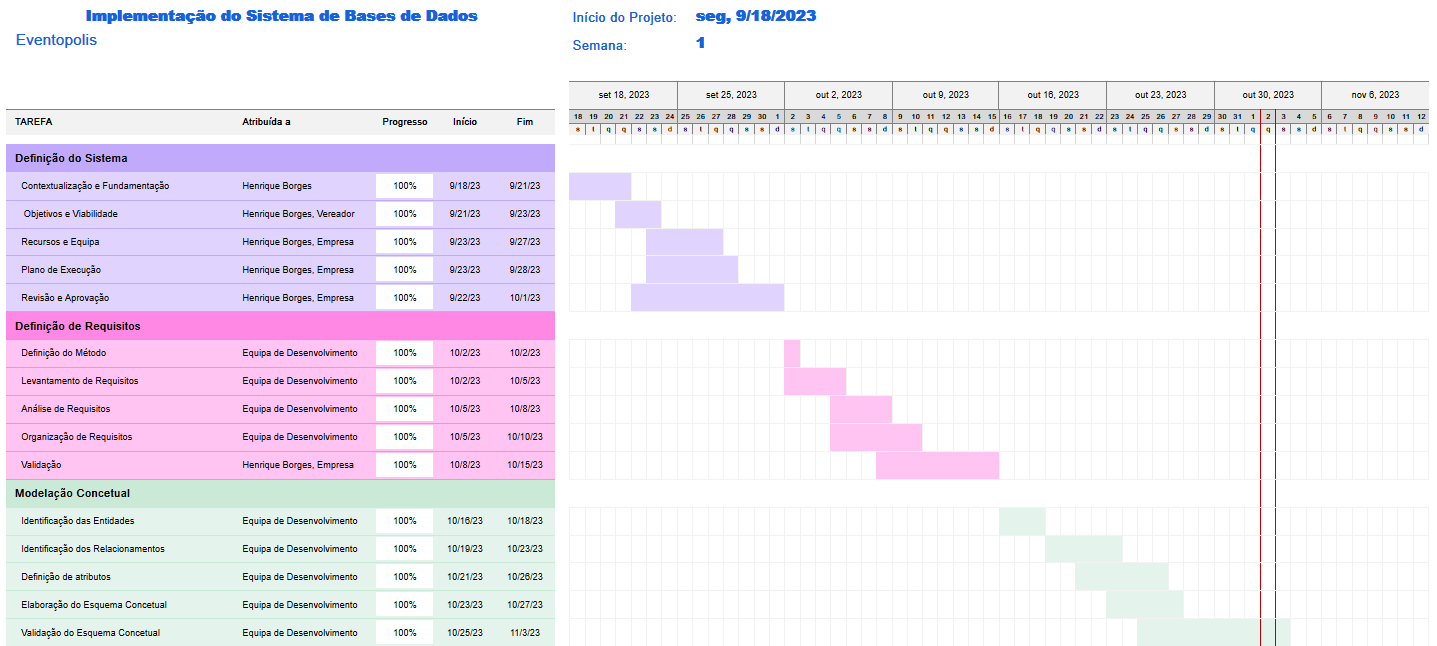
\includegraphics[width=4.5in]{images/GANTT1_c1.png}
            \caption{Diagrama de GANTT com conteúdos da primeira fase do Trabalho}
        \end{figure}
\end{frame}

\begin{frame}{Plano de Execução do Trabalho}
\begin{figure}[h]
            \centering
            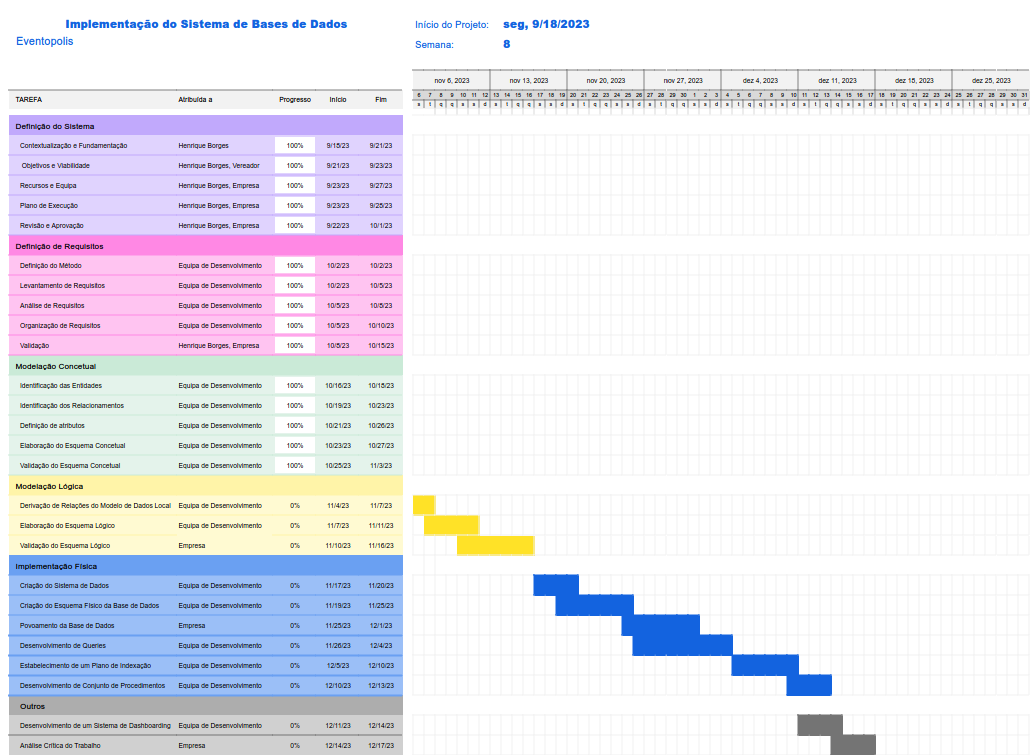
\includegraphics[width=3.75in]{images/GAANT1_c2.png}
            \caption{Diagrama de GANTT com conteúdos da segunda fase do Trabalho}
        \end{figure}
\end{frame}

\subsection{Definição de Requisitos}

\subsubsection{Método de Levantamento e de Análise de Requisitos Adotado}
\begin{frame}{Método de Levantamento e de Análise de Requisitos Adotado}
\begin{block}{Metodologia}
Com o objetivo de determinar os objetivos a serem alcançados pelo sistema de bases de dados,
foram agendadas diversas reuniões com o Prof.\ Dr.\ Henrique Borges, onde foram discutidas várias
questões pertinentes. No final destas reuniões, é previsto obter-se uma compreensão abrangente
dos requisitos a serem implementados.

\end{block}
\end{frame}

\subsubsection{Organização dos Requisitos Levantados}

\begin{frame}{Requisitos de Descrição}

\begin{table}[h]
        \centering
        \resizebox{\textwidth}{!}{%
        \begin{tabular}{ | c | c |p{10.5cm} | c | c | c |}
        \hline
        Nr & Hour & Description & Source & Analist & Type \\ \hline
        1 & 12:29 & Each event must have an unique identifier. & Henrique Borges & Aurora Matrix & DR \\ \hline
        2 & 12:29 & Each event must have an unique name & Henrique Borges & Aurora Matrix & DR \\ \hline
        3 & 12:29 & Each event must have a description & Henrique Borges & Aurora Matrix & DR \\ \hline
        4 & 12:29 & Each event must have a beginning and ending date & Henrique Borges & Aurora Matrix & DR \\ \hline
        5 & 12:29 & Each event must have a maximum capacity & Henrique Borges & Aurora Matrix & DR \\ \hline
        6 & 12:30 & There are no concurrent events & Henrique Borges & Aurora Matrix & DR \\ \hline
        7 & 12:30 & Each employee must have an unique identifier which is formatted as ""XXXXXYYYYY"" where XXXXX is a descriptor of rank or function and YYYYY is a number & Henrique Borges & Aurora Matrix & DR \\ \hline
        8 & 12:30 & Each employee must have a name & Henrique Borges & Aurora Matrix & DR \\ \hline
        9 & 12:30 & Each employee must have a VAT & Henrique Borges & Aurora Matrix & DR \\ \hline
        10 & 12:30 & Each employee must have a birth date & Henrique Borges & Aurora Matrix & DR \\ \hline
        11 & 12:30 & Each employee must have a list of emails & Henrique Borges & Aurora Matrix & DR \\ \hline
        12 & 12:30 & Each employee must have a list of phone numbers & Henrique Borges & Aurora Matrix & DR \\ \hline
        13 & 12:30 & Each employee must have an address & Henrique Borges & Aurora Matrix & DR \\ \hline
        14 & 12:30 & "An address is a composite of Street name, Locale and Postal Code" & Henrique Borges & Aurora Matrix & DR \\ \hline
        15 & 12:31 & Each sale must have an unique identifier & Henrique Borges & Aurora Matrix & DR \\ \hline
        16 & 12:31 & Each sale must have a total sale value which is the result of a certain calculation & Henrique Borges & Aurora Matrix & DR \\ \hline
        17 & 12:31 & Each sale must have the quantity of products & Henrique Borges & Aurora Matrix & DR \\ \hline
        18 & 12:31 & Each sale must have the date the sale closed & Henrique Borges & Aurora Matrix & DR \\ \hline
        19 & 12:32 & Each participant must have an unique identifier & " Henrique Borges" & Aurora Matrix & DR \\ \hline
        20 & 12:32 & Each participant must have a name & Henrique Borges & Aurora Matrix & DR \\ \hline
        \end{tabular}%
    }
    \caption{Requisitos de Descrição}
    \end{table}
\end{frame}

\begin{frame}{Requisitos de Descrição}
\begin{table}[h]
        \centering
        \resizebox{\textwidth}{!}{%
        \begin{tabular}{ | c | c |p{10.5cm} | c | c | c |}
        \hline
        21 & 12:32 & Each participant must have date of birth & Henrique Borges & Aurora Matrix & DR \\ \hline
        22 & 12:32 & Each participant must have a list of phone numbers & Henrique Borges & Aurora Matrix & DR \\ \hline
        23 & 12:32 & "Each participant must have, optionally, a list of emails" & Henrique Borges & Aurora Matrix & DR \\ \hline
        24 & 12:32 & "Each participant must have, optionally, their VAT" & Henrique Borges & Aurora Matrix & DR \\ \hline
        25 & 12:32 & "Each participant must have optionally, address" & Henrique Borges & Aurora Matrix & DR \\ \hline
        26 & 12:33 & Each product must have an unique identifier & Henrique Borges & Aurora Matrix & DR \\ \hline
        27 & 12:33 & Each product must have an unique name & Henrique Borges & Aurora Matrix & DR \\ \hline
        28 & 12:33 & Each product must have a current price & Henrique Borges & Aurora Matrix & DR \\ \hline
        29 & 12:33 & Each product must have a stock which is a number that represents the total quantity of a given product in storage & Henrique Borges & Aurora Matrix & DR \\ \hline
        30 & 12:33 & Each product must have a description & Henrique Borges & Aurora Matrix & DR \\ \hline
        31 & 12:33 & A ticket is a product who's name is the same as the event's name & Henrique Borges & Aurora Matrix & DR \\ \hline
        32 & 12:34 & Each supplier must have an unique identifier & Henrique Borges & Aurora Matrix & DR \\ \hline
        33 & 12:34 & Each supplier must have an unique name & Henrique Borges & Aurora Matrix & DR \\ \hline
        34 & 12:34 & Each supplier must have an IBAN & Henrique Borges & Aurora Matrix & DR \\ \hline
        35 & 12:34 & Each supplier must have an list of emails & Henrique Borges & Aurora Matrix & DR \\ \hline
        36 & 12:34 & Each supplier must have an list of cellphones & Henrique Borges & Aurora Matrix & DR \\ \hline
        37 & 12:34 & Each supplier must have an address & Henrique Borges & Aurora Matrix & DR \\ \hline
        38 & 12:34 & "The only type of identifier that should be manually inserted is the employee identifier, every other should be an automatic number" & Henrique Borges & Aurora Matrix & DR \\ \hline
        \end{tabular}%
    }
    \end{table}
\end{frame}

\begin{frame}{Requisitos de Descrição}
\begin{table}[h]
        \centering
        \resizebox{\textwidth}{!}{%
        \begin{tabular}{ | c | c |p{10.5cm} | c | c | c |}
        \hline
        65 & 13:01 & The amount of tickets does not exceed the maximum capacity of an event & Henrique Borges & Aurora Matrix & DR \\ \hline
        70 & 13:07 & The value of a product in a sale is dependant on it's base price at the moment of purchase and the desired quantity & Henrique Borges & Aurora Matrix & DR \\ \hline
        79 & 13:23 & Administrator info must be stored in the database as employees. & Henrique Borges & Aurora Matrix & DR \\ \hline
        81 & 13:24 & The value of a sale is sum of the value times the quantity of all products in a sale. & Henrique Borges & Aurora Matrix & DR \\ \hline
        85 & 13:28 & It must be possible to differenciate completed deliveries from ongoing reservations & Henrique Borges & Aurora Matrix & DR \\ \hline
        86 & 13:28 & It must be possible to differenciate failed reservations from ongoing reservations or completed reservations & Henrique Borges & Aurora Matrix & DR \\ \hline
    \end{tabular}%
    }
    %\caption{Requisitos de Descrição}
    \end{table}
\end{frame}

\begin{frame}{Requisitos de Manipulação}
\begin{table}[!ht]
        \centering
        \resizebox{\textwidth}{!}{%
        \begin{tabular}{ | c | c |p{10.5cm} | c | c | c |}
        \hline
        Nr & Hour & Description & Source & Analist & Type \\ \hline
        43 & 12:37 & It must be possible to consult who is the manager of an employee. & Henrique Borges & Aurora Matrix & ER \\ \hline
        44 & 12:39 & It must be possible to consult products in a sale & Henrique Borges & Aurora Matrix & ER \\ \hline
        45 & 12:41 & It must be possible to consult every closed sale & Henrique Borges & Aurora Matrix & ER \\ \hline
        46 & 12:42 & It must be possible to consult all participants in a given event & Henrique Borges & Aurora Matrix & ER \\ \hline
        47 & 12:43 & It must be possible to consult all participants in the system & Henrique Borges & Aurora Matrix & ER \\ \hline
        48 & 12:44 & It must be possible to consult the participant associated with a given sale & Henrique Borges & Aurora Matrix & ER \\ \hline
        49 & 12:45 & It must be possible to consult all products in stock & Henrique Borges & Aurora Matrix & ER \\ \hline
        50 & 12:46 & It must be possible to consult all suppliers of a given product & Henrique Borges & Aurora Matrix & ER \\ \hline
        51 & 12:46 & It must be possible to consult only past suppliers of a given product & Henrique Borges & Aurora Matrix & ER \\ \hline
        52 & 12:46 & It must be possible to consult only eventual suppliers of a given product & Henrique Borges & Aurora Matrix & ER \\ \hline
        53 & 12:47 & It must be possible to consult all of a participant's purchases & Henrique Borges & Aurora Matrix & ER \\ \hline
        54 & 12:48 & It must be possible to consult all suppliers & Henrique Borges & Aurora Matrix & ER \\ \hline
        55 & 12:49 & It must be possible to consult all employees & Henrique Borges & Aurora Matrix & ER \\ \hline
        56 & 12:50 & It must be possible to consult all events & Henrique Borges & Aurora Matrix & ER \\ \hline
        57 & 12:51 & It must be possible to consult the value of sales in a particular day & Henrique Borges & Aurora Matrix & ER \\ \hline
        58 & 12:51 & It must be possible to consult the volume of sales in a particular day & Henrique Borges & Aurora Matrix & ER \\ \hline
        59 & 12:52 & It must be possible to determine who is the participant with highest volume of sales & Henrique Borges & Aurora Matrix & ER \\ \hline
    \end{tabular}%
}
\end{table}
\end{frame}

\begin{frame}{Requisitos de Manipulação}
\begin{table}[!ht]
        \centering
        \resizebox{\textwidth}{!}{%
        \begin{tabular}{ | c | c |p{11cm} | c | c | c |}
        \hline
        60 & 12:53 & It must be possible to determine the event with the highest volume of sales. & Henrique Borges & Aurora Matrix & ER \\ \hline
        61 & 12:54 & It must be possible to determine the event with the highest rate of participation & Henrique Borges & Aurora Matrix & ER \\ \hline
        62 & 12:55 & "When the system closes, it must dump a sales report as a text file" & Henrique Borges & Aurora Matrix & ER \\ \hline
        63 & 12:59 & A participant is inserted into the database when they buy a ticket & Henrique Borges & Aurora Matrix & ER \\ \hline
        64 & 13:00 & If an event is open-entry the sale of a ticket is still registered with 0 value & Henrique Borges & Aurora Matrix & ER \\ \hline
        68 & 13:05 & It must be possible to consult what events occured in a given timespan & Henrique Borges & Aurora Matrix & ER \\ \hline
        69 & 13:06 & It must be possible to consult which employee sold the most tickets for a given event. & Henrique Borges & Aurora Matrix & ER \\ \hline
        73 & 13:16 & It must be possible to consult the events in which someone participated in & Henrique Borges & Aurora Matrix & ER \\ \hline
        74 & 13:17 & It must be possible to insert new events into the database & Henrique Borges & Aurora Matrix & ER \\ \hline
        75 & 13:18 & It must be possible to insert new employees in to the database & Henrique Borges & Aurora Matrix & ER \\ \hline
        76 & 13:19 & A product, if it exists, must be updated as soon as the supplying is concluded & Henrique Borges & Aurora Matrix & ER \\ \hline
        77 & 13:20 & A product, if new, must be added to the database as soon as it is ordered & Henrique Borges & Aurora Matrix & ER \\ \hline
        82 & 13:24 & It must be possible to consult the employee managed by another employee. & Henrique Borges & Aurora Matrix & ER \\ \hline
        83 & 13:25 & It must be possible to determine the participant with highest value of sales. & Henrique Borges & Aurora Matrix & ER \\ \hline
        84 & 13:27 & It must be possible to determine the event with highest value in sales. & Henrique Borges & Aurora Matrix & ER \\ \hline
        87 & 13:30 & It must be possible to consult all sales made by an employee & Henrique Borges & Aurora Matrix & ER \\ \hline
    \end{tabular}%
}
\end{table}
\end{frame}

\begin{frame}{Requisitos de Controlo}
        \begin{table}[h]
        \centering
        \resizebox{\textwidth}{!}{%
        \begin{tabular}{|l|l| p{10cm}|l|l|l|}
        \hline
        Nr & Hour & Description & Source & Analist & Type \\ \hline
        39 & 12:35 & Henrique Borges is a System Administrator & Henrique Borges & Aurora Matrix & AR \\ \hline
        40 & 12:36 & Maria Ivanovna Ivanova is a System Administrator & Henrique Borges & Aurora Matrix & AR \\ \hline
        41 & 12:36 & Herr Mustermann is a System Administrator & Henrique Borges & Aurora Matrix & AR \\ \hline
        42 & 12:36 & There must be a special way of accessing the database called guest for anyone who wishes to view information on events & Henrique Borges & Aurora Matrix & AR \\ \hline
        66 & 13:02 & Access to the database is only available from 07:00 to 02:00 & Henrique Borges & Aurora Matrix & AR \\ \hline
        67 & 13:04 & Database Administrators may revoke access to the database if provided with a suitable/legal reason. & Henrique Borges & Aurora Matrix & AR \\ \hline
        71 & 13:08 & An administrator has access to any and all information in the database & Henrique Borges & Aurora Matrix & AR \\ \hline
        72 & 13:09 & An administrator has access to all and any functionalities of the database & Henrique Borges & Aurora Matrix & AR \\ \hline
        78 & 13:23 & Only administrators may update information & Henrique Borges & Aurora Matrix & AR \\ \hline
        80 & 13:23 & Only administrators have access to the total value of sales & Henrique Borges & Aurora Matrix & AR \\ \hline
        88 & 13:30 & The usernames in the database correspond directly to the identifier & Henrique Borges & Aurora Matrix & AR \\ \hline
        \end{tabular}
        }
        \end{table}
\end{frame}

\subsubsection{Análise e Validação Geral dos Requisitos}
\begin{frame}{Análise e Validação Geral dos Requisitos}
Depois do levantamento dos requisitos, marcou-se uma reunião no intuito de o pessoal interno tomar conhecimento dos requisitos documentados.

Esta reunião, por sua vez, foi realizada com sucesso, e o pessoal interno mostrou-se satisfeito com o progresso e nível de detalhe a que os membros da equipa de desenvolvimento de BD chegaram, especialmente o Prof.\ Dr.\ Henrique Borges, que viu muito potencial neste projeto.
\end{frame}

\subsection{Modelação Concetual}
\subsubsection{Identificação e Caracterização das Entidades e dos Atributos das mesmas}
\begin{frame}{Identificação e Caracterização das Entidades e dos Atributos das mesmas}
\begin{itemize}
                 \item{\textbf{Evento:}} Evento a ser gerido. 
                     \begin{itemize}
                     \item{ID:} Chave Primária da entidade que estará no domínio INTEGER
                       e será auto incrementável;
                     \item{Nome:} O nome de um evento que estará no domínio VARCHAR(75).
                     \item{Descrição:} A descrição de um elemento da tabela ``Evento'' será
                       um breve texto que introduz o tema e qualquer tipo de subevento que possa
                       estar inserido no evento. Sendo assim, este atributo estará no domínio TEXT;
                     \item{DataFim:} A data do fim de um evento será uma data com as horas a qual
                       o evento será dado por oficialmente terminado. Sendo assim, estará no domínio
                       DATETIME;
                     \item{DataInicio:} A data do inicio de um evento será uma data com as horas a qual
                       o evento será dado por oficialmente iniciado. Sendo assim, estará no domínio
                       DATETIME;
                     \item{Capacidade:} É importante ter noção da quantidade máxima de participantes num
                       dado evento. Então, este atributo será um elemento numérico e estará no domínio INTEGER.
                     \end{itemize}
\end{itemize}
\end{frame}
\begin{frame}{Identificação e Caracterização das Entidades e dos Atributos das mesmas}
\begin{itemize}
                 \item{\textbf{Funcionário:}} Colaborador da câmara munincipal.
                     \begin{itemize}
                     \item{ID:} Chave Primária da entidade que estará no domínio VARCHAR(10);
                     \item{Nome:} O nome legal ou social de um funcionário também será armazenado e estará
                       no domínio VARCHAR(75);
                     \item{NIF:} O número de identificação fiscal é um número de 9 algarismos e, portanto estará
                       no domínio VARCHAR(9);
                     \item{DataNascimento:} Data de nascimento que estará no domínio DATE;
                       
                     \item{Email:} Email é um atributo multivalorado que estará no domínio VARCHAR(75);
                       
                     \item{NTelemovel:} Números de telemóvel. Podem conter letras e números. É um atributo multivalorado no domínio VARCHAR(20);
                       
                     \item{Morada:} Morada composta por rua, localidade, código-postal. Atributo Composto de VARCHAR(), onde rua será VARCHAR(50), localidade VARCHAR(30) e código-postal VARCHAR(15);
                       
                     \end{itemize}
\end{itemize}
\end{frame}
\begin{frame}{Identificação e Caracterização das Entidades e dos Atributos das mesmas}
\begin{itemize}
                 \item{\textbf{Participante:}} Pessoa que participa num evento(s). É registado no sistema quando efetua a compra do seu primeiro bilhete para um evento;
                     \begin{itemize}
                     \item{ID:} Chave Primária da entidade que estará no domínio INTEGER;
                       
                     \item{Nome:} O nome legal ou social da pessoa também será armazenado e estará
                       no domínio VARCHAR(75);
                       
                     \item{NIF:} O número de identificação fiscal é um número de 9 algarismos e, portanto estará no domínio VARCHAR(9). Este campo é opcional;
                       
                     \item{DataNascimento:} Data de nascimento que estará no domínio DATE;
                       
                     \item{Email:} Email do participante que estará no domínio. É um atributo multivalorado no domínio VARCHAR(75). Este campo é opcional;
                       
                     \item{NTelemovel:} Números de telemóvel. Podem conter letras e números. É também um atributo multivalorado no domínio VARCHAR(20);
                       
                     \item{Morada:} Morada composta por rua, localidade, código-postal. Atributo Composto de VARCHAR(), onde rua será VARCHAR(50), localidade VARCHAR(30) e código-postal VARCHAR(15). Este campo é opcional;
                       
                     \end{itemize}
\end{itemize}
\end{frame}
\begin{frame}{Identificação e Caracterização das Entidades e dos Atributos das mesmas}
\begin{itemize}
                 \item{\textbf{Artigo:}} Artigo que é possível estar numa venda;
                     \begin{itemize}
                     \item{ID:} Chave Primária da entidade que estará no domínio INTEGER;
                       
                     \item{Nome:} O nome do artigo que estará no domínio VARCHAR(75);
                       
                     \item{Descrição:} A descrição de um elemento da tabela ``Artigo'' será
                       um breve texto que descreve o produto em questão e qualquer medida extra necessária a ter com o mesmo. Sendo assim, este atributo estará no domínio TEXT;
                       
                     \item{Preço:} Valor de um artigo, logo estará no domínio DECIMAL(5,2);
                       
                     \item{Stock:} Quantidade de um artigo que está disponível, estará no domínio INTEGER;
                       
                     \end{itemize}
\end{itemize}
\end{frame}
\begin{frame}{Identificação e Caracterização das Entidades e dos Atributos das mesmas}
\begin{itemize}
                 \item{\textbf{Venda:}} Venda de artigo(s) a ser efetuada a um participante por parte de um funcionário;
                     \begin{itemize}
                     \item{ID:} Chave Primária da entidade que estará no domínio INTEGER;
                       
                     \item{Valor:} Valor total da venda que estará no domínio DECIMAL(5,2);
                       
                     \item{Quantidade:} Valor total do número de artigos na venda que estará no domínio INTEGER;
                       
                     \item{Data:} Data na qual a venda aconteceu, logo estará no domínio DATE;
                       
                     \end{itemize}
\end{itemize}
\end{frame}
\begin{frame}{Identificação e Caracterização das Entidades e dos Atributos das mesmas}
\begin{itemize}
                 \item{\textbf{Fornecedor:}} Quem fornece os artigos;
                     \begin{itemize}
                     \item{ID:} Chave Primária da entidade que estará no domínio INTEGER;
                       
                     \item{Nome:} O nome da empresa fornecedora que estará no domínio VARCHAR(75);
                       
                     \item{IBAN:} Código de identificação de conta bancária para a qual devem ser feitos os pagamentos ao fornecedor. Está no domínio VARCHAR(50);
                       
                     \item{Email:} Email do fornecedor que estará no domínio. É um atributo multivalorado no domínio VARCHAR(75);
                       
                     \item{Contacto:} Pessoa que representa a empresa e o seu número de telemóvel, estará no domínio VARCHAR(50);
                       
                     \item{NTelemovel:} Números de telemóvel. Podem conter letras e números. É também um atributo multivalorado no domínio VARCHAR(20);
                       
                     \item{Morada:} Morada composta por rua, localidade, código-postal. Atributo Composto de VARCHAR(), onde rua será VARCHAR(50), localidade VARCHAR(30) e código-postal VARCHAR(15);
                       
                     \end{itemize}
\end{itemize}
\end{frame}


\subsubsection{Identificação e Caracterização da Associação dos Atributos com as Entidades e Relacionamentos e dos Atributos das mesmas}
\begin{frame}{Identificação e Caracterização da Associação dos Atributos com as Entidades e Relacionamentos e dos Atributos das mesmas}
\begin{itemize}
                 \item{\textbf{Evento emprega Funcionário}:} Relacionamento entre Evento e Funcionário, representado quais funcionários estão alocados para quais eventos. Sendo a cardinalidade muitos para muitos;
                 \item{\textbf{Funcionário gere Funcionário}:} Relacionamento entre Funcionário e Funcionário, representado qual funcionário gere qual/quais funcionários são geridos por um Funcionário. Sendo a cardinalidade um para muitos;
                 \item{\textbf{Funcionário realiza Venda}:} Relacionamento entre Funcionário e Venda, representado qual funcionário efetuou uma Venda. Sendo a cardinalidade um para muitos.
\end{itemize}
\end{frame}
\begin{frame}{Identificação e Caracterização da Associação dos Atributos com as Entidades e Relacionamentos e dos Atributos das mesmas}
\begin{itemize}
                 \item{\textbf{Venda contém Artigo}:} Relacionamento entre Venda e Artigo, representando quais artigos estão numa venda. Sendo a cardinalidade muitos para muitos.
                     \begin{itemize}
                     \item{Valor:} Valor do artigo no momento da venda, estará então no domínio DECIMAL(5,2);
                       
                     \item{Quantidade:} Valor total da quantidade de um dado artigo numa venda, estará então no domínio INTEGER;
                       
                     \end{itemize}
                 \item{\textbf{Venda para Participante}:} Relacionamento entre Venda e Participante, representando a que participante uma venda pertence. Sendo a cardinalidade 1 para muitos;
\end{itemize}
\end{frame}
\begin{frame}{Identificação e Caracterização da Associação dos Atributos com as Entidades e Relacionamentos e dos Atributos das mesmas}
\begin{itemize}
                 \item{\textbf{Artigo fornecido por Fornecedor}:} Relacionamento entre Artigo e Fornecedor, representado o fornecedor pelo qual um artigo foi fornecido. Sendo a cardinalidade muitos para muitos;
                     \begin{itemize}
                     \item{Data:} Data na qual o artigo foi entregue pelo fornecedor, estará então no domínio DATETIME;
                     \item{Quantidade:} Valor total da quantidade de um dado artigo numa entrega por parte de um fornecedor, estará então no domínio INTEGER;
                       
                     \end{itemize}
\end{itemize}
\end{frame}
\begin{frame}{Identificação e Caracterização da Associação dos Atributos com as Entidades e Relacionamentos e dos Atributos das mesmas}
\begin{itemize}
                 \item{\textbf{Artigo encomendado do Fornecedor}:} Relacionamento entre Artigo e Fornecedor, representado o fornecedor pelo qual um artigo foi encomendado. Sendo a cardinalidade muitos para muitos;
                     \begin{itemize}
                     \item{DataEncomenda:} Data na qual o artigo foi encomendado ao fornecedor, estará então no domínio DATETIME;
                     \item{DataEsperada:} Data na qual o artigo é esperado que seja entregue, estará então no domínio DATETIME. DataEncomenda e DataEsperada compõe a chave primária do relacionamento;
                     \item{Quantidade:} Valor total da quantidade de um dado artigo numa encomenda por parte de um fornecedor, estará então no domínio INTEGER;
                       
                     \end{itemize}
\end{itemize}
\end{frame}

\subsubsection{Apresentação e Explicação do Diagrama ER Produzido}
\begin{frame}{Apresentação e Explicação do Diagrama ER Produzido}
\begin{figure}[h]
            \centering
            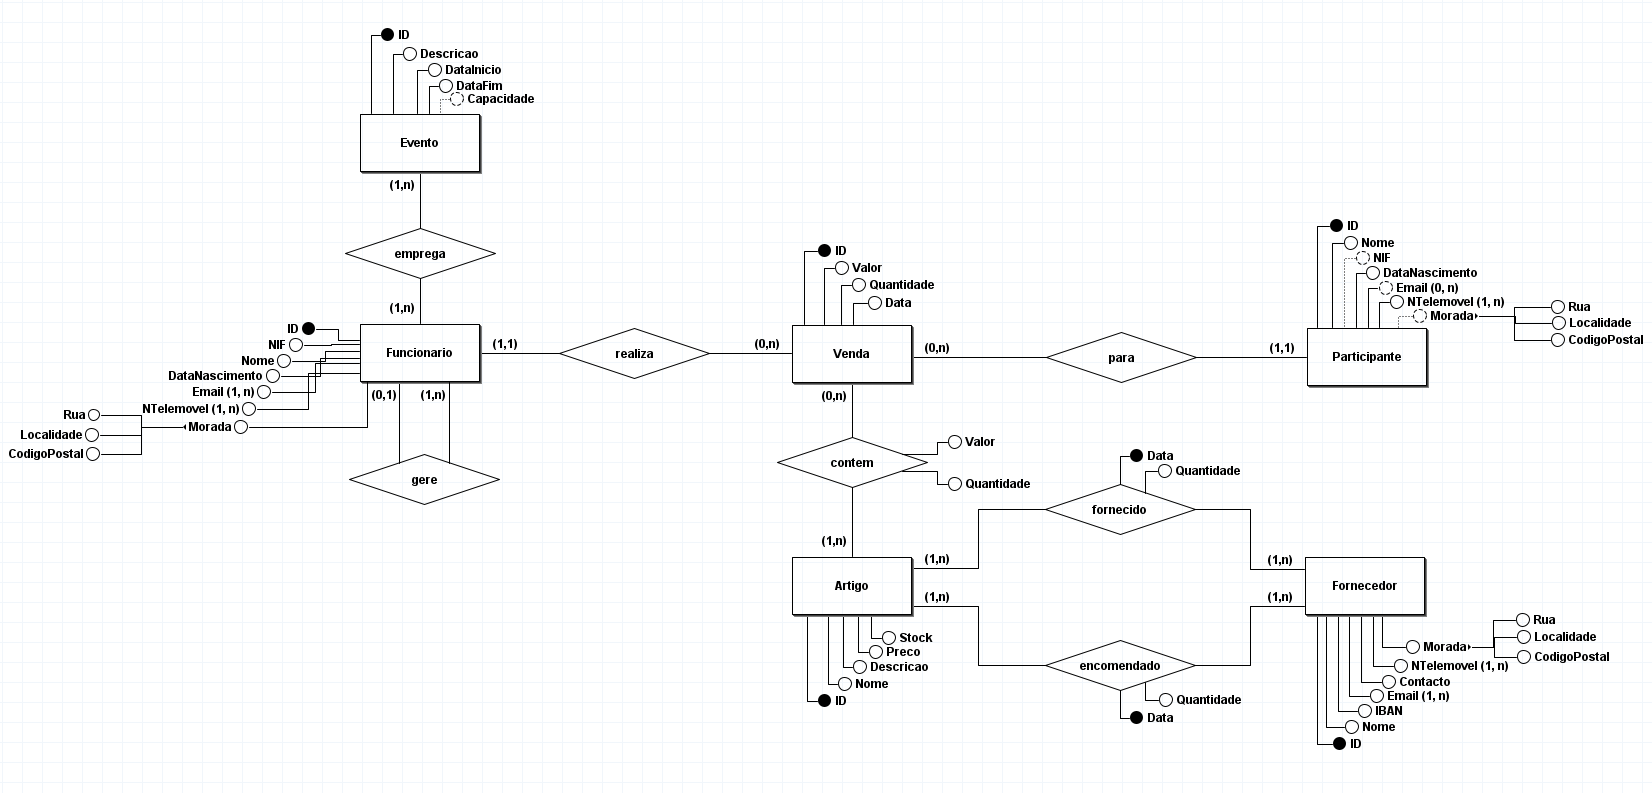
\includegraphics[width=4.7in]{images/Conceitual_Com_Atributos.png}
            %%\caption{Diagrama Conceitual}
        \end{figure}
\end{frame}

\mycomment{
\subsubsection{Justificação do Modelo Conceptual usando 5 Requisitos}
\begin{frame}{Justificação do Modelo Conceptual usando 5 Requisitos}

\begin{table}[!ht]
    \centering
    \resizebox{\columnwidth}{!}{%
    \begin{tabular}{|l|l|l|>{\raggedright\arraybackslash}p{8cm}|l|l|l|}
    \hline
        Nr & ~ & Data e Hora & Descrição & Área & Fonte & Analista \\ \hline
    RD06 & 6 & 12:34 & Cada fornecedor deve ter um identificador, nome, IBAN, email, contacto (a pessoa que contactamos na empresa e o seu número de telemóvel), lista de números de telemóvel, morada (rua, localidade, código-postal) & Eventos & Henrique Borges & Aurora Matrix \\ \hline
    
    RM17 & 26 & 12:53 & O administrador deve ser capaz de consultar os passados fornecedores de um certo artigo & Eventos & Henrique Borges & Aurora Matrix \\ \hline
    RM02 & 11 & 12:38 & Um funcionário deve ser capaz de consultar qual é o funcionário que o gere & Eventos & Henrique Borges & Aurora Matrix \\ \hline
    
     RM23 & 32 & 12:59 & Deve ser possível determinar qual é o evento com maior volume de vendas & Eventos & Henrique Borges & Aurora Matrix \\ \hline

     RM33 & 45 & 13:13 & O administrador deve ser capaz de consultar qual foi o funcionário que vendeu mais bilhetes num dado evento & Eventos & Henrique Borges & Aurora Matrix \\ \hline
     
    \end{tabular}}%
\end{table}
\end{frame}
}

\subsection{Modelação Lógica}

\subsubsection{Construção e Validação do Modelo de Dados Lógico}
\begin{frame}{Construção e Validação do Modelo de Dados Lógico}
Com a modelação conceptual completa e validada, a equipa de desenvolvimento procedeu com a modelação
lógica do SBD, sendo que a mesma é uma tradução direta do modelo conceptual, introduzindo agora chaves estrangeiras.
\end{frame}

\subsubsection{Normalização de Dados}
\begin{frame}{Normalização de Dados}
Devido à abordagem que adotámos no trabalho desde o modelo conceptual onde a leitura ocorre da esquerda para a direita e de cima para baixo, e considerando que atendemos a todos os requisitos das leis de normalização, os nossos dados encontram-se naturalmente normalizados na Terceira Forma Normal (3FN).

O facto de estarem normalizados em 3FN proporciona várias vantagens, incluindo a prevenção de anomalias como a redundância, 
e problemas de consistência decorrentes de processos de inserção, atualização ou remoção. 
Além disso, evita a atualização deficiente de um determinado registo com múltiplas ocorrências, onde nem todas são corretamente atualizadas.
\end{frame}

\subsubsection{Apresentação e Explicação do Modelo Lógico Produzido}
\begin{frame}{Apresentação e Explicação do Modelo Lógico Produzido}
\textbf{Tradução de Entidades}
    \begin{itemize}
        \item{\textbf{Evento $\rightarrow$ EventCal}}
            \begin{itemize}
                \item{ID $\rightarrow$ EventID}
                \item{Nome $\rightarrow$ EventName}
                \item{Descricao $\rightarrow$ EventDescription}
                \item{DataInicio $\rightarrow$ EventStart}
                \item{DataFim $\rightarrow$ EventEnd}
                \item{Capacidade $\rightarrow$ Capacity}
            \end{itemize}
        \item{\textbf{Funcionário $\rightarrow$ Employee}}
            \begin{itemize}
                \item{ID $\rightarrow$ EmployeeID}
                \item{Nome $\rightarrow$ EmployeeName}
                \item{NIF $\rightarrow$ EmployeeVAT}
                \item{DataNascimento $\rightarrow$ EmployeeBirthDate}
            \end{itemize}
    \end{itemize}
\end{frame}

\begin{frame}{Apresentação e Explicação do Modelo Lógico Produzido}
            Temos dois atributos multivalorados na entidade Funcionário que geram duas novas tabelas:
            \begin{itemize}
                \item{\textbf{Email $\rightarrow$ EmployeeEmail}}
                    \begin{itemize}
                        \item{EmployeeID\_eem:} Chave estrangeira (chave primária e NOT NULL) que referencia a chave candidata EmployeeID na tabela Employee.
                        \item{Email:} Atributo que representa um email tal como no modelo conceptual.
                    \end{itemize}
                \item{\textbf{NTelemovel $\rightarrow$ EmployeePhone}}
                    \begin{itemize}
                        \item{EmployeeID\_ep:} Chave estrangeira (chave primária e NOT NULL) que referencia a chave candidata EmployeeID na tabela Employee.
                        \item{Phone:} Atributo que representa um número de telemóvel como no modelo conceptual.
                    \end{itemize}
            \end{itemize}
\end{frame}

\begin{frame}{Apresentação e Explicação do Modelo Lógico Produzido}
        \begin{itemize}
        \item{\textbf{Venda $\rightarrow$ Sale}}
            \begin{itemize}
                \item{ID $\rightarrow$ ReceiptNO}
                \item{Valor $\rightarrow$ TotalValue}
                \item{Quantidade $\rightarrow$ TotalQuantity}
                \item{Data $\rightarrow$ DateOfSale}
                \item{EmployeeID\_s:} Chave estrangeira (NOT NULL) que referencia a chave candidata EmployeeID na tabela Employee.
                \item{ParticipantID\_s:} Chave estrangeira (NOT NULL) que referencia a chave candidata ParticipantID na tabela Participant.
            \end{itemize}
        \item{\textbf{Participante $\rightarrow$ Participant}}
            \begin{itemize}
                \item{ID $\rightarrow$ ParticipantID}
                \item{Nome $\rightarrow$ ParticipantName}
                \item{NIF $\rightarrow$ ParticipantVAT}
                \item{DataNascimento $\rightarrow$ ParticipantBirthDate}
                \item{Rua $\rightarrow$ Street}
                \item{Localidade $\rightarrow$ Locale}
                \item{CodigoPostal $\rightarrow$ Postal}
            \end{itemize}
        \end{itemize}
\end{frame}

\begin{frame}{Apresentação e Explicação do Modelo Lógico Produzido}
            Temos dois atributos multivalorados na entidade Participante que geram duas novas tabelas:
            \begin{itemize}
                \item{\textbf{NTelemovel $\rightarrow$ ParticipantPhone}}
                    \begin{itemize}
                        \item{ParticipantID\_pp:} Chave estrangeira (chave primária e NOT NULL) que referencia 
                        a chave candidata ParticipantID na tabela Participant.
                        \item{Phone:} Atributo que representa um número de telemóvel como no modelo conceptual.
                    \end{itemize}
                \item{\textbf{Email $\rightarrow$ ParticipantEmail}}
                    \begin{itemize}
                        \item{ParticipantID\_pem:} Chave estrangeira (chave primária e NOT NULL) que referencia a chave candidata ParticipantID na tabela Participant.
                        \item{Email:} Atributo que representa um email como no modelo conceptual.
                    \end{itemize}
            \end{itemize}
\end{frame}

\begin{frame}{Apresentação e Explicação do Modelo Lógico Produzido}
    \begin{itemize}
        \item{\textbf{Artigo $\rightarrow$ Produto}}
            \begin{itemize}
                \item{ID $\rightarrow$ ProductID}
                \item{Nome $\rightarrow$ ProductName}
                \item{Descricao $\rightarrow$ ProductDescription}
                \item{Preco $\rightarrow$ BasePrice}
                \item{Stock $\rightarrow$ QuantityInStock}
            \end{itemize}
        \item{\textbf{Forncedor $\rightarrow$ Supplier}}
            \begin{itemize}
                \item{ID $\rightarrow$ SupplierID}
                \item{Nome $\rightarrow$ SupplierName}
                \item{IBAN $\rightarrow$ IBAN}
                \item{Rua $\rightarrow$ Street}
                \item{Localidade $\rightarrow$ Locale}
                \item{CodigoPostal $\rightarrow$ Postal}
            \end{itemize}
    \end{itemize}
\end{frame}

\begin{frame}{Apresentação e Explicação do Modelo Lógico Produzido}
             Temos dois atributos multivalorados na entidade Artigo que geram duas novas tabelas:
             \begin{itemize}
                \item{\textbf{NTelemovel $\rightarrow$ SupplierPhone}}
                    \begin{itemize}
                        \item{SupplierID\_sp:} Chave estrangeira (chave primária e NOT NULL) que referencia a chave candidata SupplierID
                        na tabela Supplier.
                        \item{Phone:} Atributo que representa um número de telemóvel como no modelo conceptual.
                    \end{itemize}
                \item{\textbf{Email $\rightarrow$ SupplierEmail}}
                    \begin{itemize}
                        \item{SupplierID\_sem:} Chave estrangeira (chave primária e NOT NULL) que referencia a chave candidata SupplierID na tabela Supplier.
                        \item{Email:} Atributo que representa um email como no modelo conceptual.
                    \end{itemize}
            \end{itemize}    
\end{frame}

\begin{frame}{Apresentação e Explicação do Modelo Lógico Produzido}
    \textbf{Tradução de Relacionamentos}
    
    Os relacionamentos com cardinalidade \textit{n} para \textit{n} geram novas tabelas. Veremos como são traduzidos os mesmos.
    \begin{itemize}
        \item{\textbf{Evento emprega Funcionário $\rightarrow$ EventEmployee}}
            \begin{itemize}
                \item{EventID\_ee:} Chave estrangeira (chave primária composta com EmployeeID\_ee) que referencia a chave candidata EventID na tabela EventCal.
                \item{EmployeeID\_ee:} Chave estrangeira (chave primária composta com EventID\_ee) que referencia a chave candidata EmployeeID na tabela Employee.
            \end{itemize}
    \end{itemize}
\end{frame}

\begin{frame}{Apresentação e Explicação do Modelo Lógico Produzido}
    \begin{itemize}
        \item{\textbf{Venda contém Artigo $\rightarrow$ SaleProduct}}
            \begin{itemize}
                \item{ReceiptNO\_sp:} Chave estrangeira (chave primária composta com ProductID\_sp) 
                que referencia a chave candidata ReceiptNO na tabela Sale.
                \item{ProductID\_sp:} Chave estrangeira que (chave primária composta com ReceiptNO\_sp)
                referencia a chave candidata ProductID na tabela Product.
                \item{Valor $\rightarrow$ CurrentValue}
            \end{itemize}
        \item{\textbf{Artigo fornecido por Fornecedor $\rightarrow$ ProductSupplierPast}}
            \begin{itemize}
                \item{ProductID\_psp:} Chave estrangeira (chave primária composta com SupplierID\_psp e DateOfDelivery)
                que referencia a chave candidata ProductID na tabela Product.
                \item{SupplierID\_psp:} Chave estrangeira (chave primária composta com ProductID\_psp e DateOfDelivery)
                que referencia a chave candidata SupplierID na tabela Supplier.
                \item{Data $\rightarrow$ DateOfDelivery:} Chave primária composta com ProductID\_psp e SupplierID\_psp. 
                \item{Quantidade $\rightarrow$ Quantity}
            \end{itemize}
    \end{itemize}
\end{frame}

\begin{frame}{Apresentação e Explicação do Modelo Lógico Produzido}
    \begin{itemize}
        \item{\textbf{Artigo encomendado a Fornecedor $\rightarrow$ ProductSupplierFuture}}
            \begin{itemize}
                \item{ProductID\_psf:} Chave estrangeira (chave primária composta com SupplierID\_psf, 
                DateOfReservation e DateOfSchedule) que referencia a chave candidata ProductID na tabela Product.
                \item{SupplierID\_psf:} Chave estrangeira (chave primária composta com ProductID\_psf,
                DateOfReservation e DateOfSchedule) que referencia a chave candidata SupplierID na tabela Supplier.
                \item{DataEncomenda $\rightarrow$ DateOfReservation:} Chave primária composta com ProductID\_psf, SupplierID\_psf e DateOfSchedule.
                \item{DataEsperada $\rightarrow$ DateOfSchedule:} Chave primária composta com ProductID\_psf, 
                SupplierID\_psf e DateOfReservation.
                \item{Quantidade $\rightarrow$ Quantity}
            \end{itemize}
    \end{itemize}
\end{frame}

\begin{frame}{Apresentação E Explicação Do Modelo Lógico Produzido}
\begin{figure}
    \centering
    \includegraphics[width=4.7in]{images/Logico}
\end{figure}
\end{frame}

\subsubsection{Validação do Modelo com Interrogações do Utilizador}
\begin{frame}[fragile]{Validação do Modelo com Interrogações do Utilizador}
\usetikzlibrary{positioning}
\begin{itemize}
    \item{Saber qual evento teve a maior taxa de participação de todos (RM61)}
$$\tau_{rate} DESC \gamma_{ID, Name ; rate} \pi_{\delta}( (\rho_{EV}EventCal) \bowtie$$
    $$(\rho_{SP} SaleProduct)  \bowtie_{\alpha \wedge \beta}
(\rho_P Product)) $$
Sabendo que:

$\delta: EV.EventID\rightarrow ID,EV.EventName\rightarrow Name,SUM(SP.Quantity)/EV.Capacity\rightarrow rate$.

$\alpha: P.ProductID = SP.ProductID\_sp$

$\beta : P.ProductName = EV.EventName$
\end{itemize}
\end{frame}

\begin{frame}[fragile]{Validação do Modelo com Interrogações do Utilizador}
\begin{itemize}
\item{Saber qual é o evento com maior valor de vendas (RM94)}
$$\tau_{TotVal} DESC \gamma_{ID, Name; TotVal} \pi_{\delta}( (\rho_{EV} EventCal) \bowtie_{\alpha} (\rho_S Sale )$$
Onde:

$\alpha : EV.EventStart < S.DateOfSale < EV.EventEnd$

$\delta: EV.EventID\rightarrow ID, EV.EventName\rightarrow Name, SUM(S.TotalValue)\rightarrow TotVal$
\end{itemize}
\end{frame}
\subsection{Modelação Física}

\subsubsection{Tradução do Esquema Lógico para o Sistema de Gestão de Bases de Dados Escolhido}
\begin{frame}{Tradução do Esquema Lógico para o Sistema de Gestão de Bases de Dados Escolhido}
Esta tradução é direta, sendo que até se pode utilizar uma funcionalidade do \textit{MySQL Workbench} para a realizar.
Listam-se exemplos de criação de tabelas.
\end{frame}
\begin{frame}[fragile]{Criação da Tabela SaleProduct}

        Esta tabela representa o relacionamento Venda contém Artigo, onde indicamos todos os atributos como pedido no modelo lógico, bem como a identificação de chave primária composta com ReceiptNO\_sp e ProductID\_sp.
\begin{lstlisting}[language=sql]
CREATE TABLE SaleProduct (
        ReceiptNO_sp INTEGER NOT NULL,
        ProductID_sp INTEGER NOT NULL,
        CurrentValue DECIMAL(5,2) NOT NULL,
        Quantity INTEGER NOT NULL,
        PRIMARY KEY (ReceiptNO_sp, ProductID_sp),
        FOREIGN KEY (ReceiptNO_sp)
      REFERENCES Sale (ReceiptNO),
        FOREIGN KEY (ProductID_sp)
      REFERENCES Product (ProductID)
);
\end{lstlisting}
        \end{frame}
\begin{frame}[fragile]{Criação da Tabela EventCal}

        No caso da tabela EventCal, a tradução é ainda mais simples, visto que não tem chaves estrangeiras. Sendo assim, 
        só tivemos que indicar os atributos como pedido e indicar que a chave primária é EventID.
\begin{lstlisting} [language=sql]
CREATE TABLE EventCal (
        EventID INTEGER AUTO_INCREMENT,
        EventName VARCHAR(75) NOT NULL UNIQUE,
        EventDescription TEXT NOT NULL,
        EventStart DATETIME NOT NULL,
        EventEnd   DATETIME NOT NULL,
        Capacity INTEGER NOT NULL,
        PRIMARY KEY (EventID)
);
\end{lstlisting}
\end{frame}

\subsubsection{Tradu\c{c}\~{a}o das Interroga\c{c}\~{o}es do Utilizador para SQL}
\begin{frame}{Tradu\c{c}\~{a}o das  Interroga\c{c}\~{o}es do Utilizador para SQL}
Neste ponto, traduziremos alguns requisitos de manipulação em \textit{queries} de MySQL, assim como as tabelas que resultam da execução das mesmas, tendo em conta o povoamento que usamos, que se encontra nos Anexos deste relatório.
\end{frame}

\begin{frame}[fragile]{Tradu\c{c}\~{a}o das  Interroga\c{c}\~{o}es do Utilizador para SQL}
Saber qual evento teve a maior taxa de participação de todos (RM61)
\begin{lstlisting} [language=sql]
SELECT EV.EventID, 
       EV.EventName, 
       SUM(SP.Quantity) / EV.Capacity * 100 AS rate
FROM EventCal as EV INNER JOIN SaleProduct as SP
    INNER JOIN Product AS P
        ON P.ProductID = SP.ProductID_sp AND
           P.ProductName = EV.EventName
    GROUP BY EV.EventID, EV.EventName
        ORDER BY rate DESC
    LIMIT 1;
    \end{lstlisting}
    \begin{figure}[H]
            \centering
            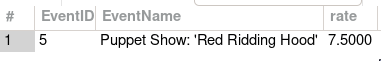
\includegraphics[width=2.5in]{images/querie1.png}
            \caption{Resultado RM61}
    \end{figure}
\end{frame}

\begin{frame}[fragile]{Tradu\c{c}\~{a}o das  Interroga\c{c}\~{o}es do Utilizador para SQL}
Saber qual é o evento com maior valor de vendas (RM94)
\begin{lstlisting} [language=sql]
SELECT E.EmployeeID, E.name, SUM(S.Val) AS totVal
FROM EventCal AS E INNER JOIN sale as S
    ON S.DateOfSale BETWEEN EV.EventStart
    AND EV.EventFin
GROUP BY E.EmployeeID, E.name
    ORDER BY totVal DESC
    LIMIT 1;
    \end{lstlisting}
    \begin{figure}[H]
            \centering
            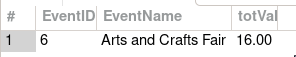
\includegraphics[width=2.5in]{images/querie2.png}
            \caption{Resultado RM94}
    \end{figure}
\end{frame}

\subsubsection{Defini\c{c}\~{a}o e Caracteriza\c{c}\~{a}o das Vistas de Utiliza\c{c}\~{a}o em SQL}
\begin{frame}{Defini\c{c}\~{a}o e Caracteriza\c{c}\~{a}o das Vistas de Utiliza\c{c}\~{a}o em SQL}

Apresentemos então algumas vistas que se definiu ao longo do desenvolvimento da BD. Vistas estas que restringem o utilizador, de obter informação além do que as vistas permitem. 
\end{frame}
\begin{frame}[fragile]{Defini\c{c}\~{a}o e Caracteriza\c{c}\~{a}o das Vistas de Utiliza\c{c}\~{a}o em SQL}
\begin{lstlisting}[language=sql]
CREATE VIEW product_supplier AS
    SELECT P.ProductID AS ProductID, 
           PSP.SupplierID_psp AS PastSupplierID,
           PSF.SupplierID_psf AS FutureSupplierID
        FROM Product AS P 
            INNER JOIN ProductSupplierPast AS PSP 
            ON P.ProductID = PSP.ProductID_psp
            INNER JOIN ProductSupplierFuture AS PSF
            ON P.ProductID = PSF.ProductID_psf
    GROUP BY P.ProductID,
             PSP.SupplierID_psp,
             PSF.SupplierID_psf;
\end{lstlisting}
\end{frame}
\begin{frame}[fragile]{Defini\c{c}\~{a}o e Caracteriza\c{c}\~{a}o das Vistas de Utiliza\c{c}\~{a}o em SQL}
\begin{lstlisting}[language=sql]
CREATE VIEW BestSellersEmployee AS
    SELECT EV.EventID AS EventID,
           S.EmployeeID_s AS EmployeeID,
           SUM(SP.Quantity) AS Quantity
        FROM EventCal AS EV 
        INNER JOIN EventEmployee AS EE
            ON EV.EventID = EE.EventID_ee
        INNER JOIN Employee AS E
            ON EE.EmployeeID_ee = E.EmployeeID
\end{lstlisting}
\end{frame}
\begin{frame}[fragile]{Defini\c{c}\~{a}o e Caracteriza\c{c}\~{a}o das Vistas de Utiliza\c{c}\~{a}o em SQL}
\begin{lstlisting}[language=sql] 
        INNER JOIN Sale AS S
            ON E.EmployeeID = S.EmployeeID_s
        INNER JOIN SaleProduct AS SP
            ON S.ReceiptNO = SP.ReceiptNO_sp
        INNER JOIN Product AS P
            ON P.ProductName = EV.EventName
    GROUP BY EV.EventID, S.EmployeeID_s
        ORDER BY SUM(SP.Quantity) DESC;
\end{lstlisting}
\end{frame}

\subsubsection{C\'{a}lculo do Espa\c{c}o da Base de Dados)}
\begin{frame}[fragile]{C\'{a}lculo do Espa\c{c}o da Base de Dados}
De forma a computar o espaço utilizado pela Base de Dados podemos utilizar a seguinte \textit{query} de MariaDB/MySQL:
\begin{lstlisting}[language=sql]
SELECT 
    table_schema 
        AS 'Database Name', 
    SUM(data_length + index_length)
        AS 'Size in Bytes', 
    ROUND(SUM(data_length + index_length) 
         / 1024 / 1024, 2) Database Name
        AS 'Size in MiB' 
    FROM information_schema.tables
    WHERE table_schema = 'mademoiselle_borges';
\end{lstlisting}
\end{frame}

\begin{frame}{C\'{a}lculo do Espa\c{c}o da Base de Dados}
Ou, alternativamente, recorrendo a uma ferramenta, como ``MySQL Workbench'', no menu contexto esquerdo, sob \textit{schemas}, clicando no símbolo
`i', conseguimos ver o espaço ocupado pelo nosso SBD.

Sendo assim, a nossa Base de Dados ocupa um total de $0.53$ \textit{Mebibytes} após o povoamento inicial.
Como podemos ver na tabela resultante da \textit{query} apresentada:\\
\begin{center}
\begin{tabular}{ |c | c | c |}
    \hline
     Database Name & Size in Bytes & Size in MebiBytes \\
     \hline
     mademoiselle\_borges & $557056$ &   $0.53$ \\ 
    \hline
\end{tabular}
\end{center}

Após fazermos o cálculo do tamanho que a Base de Dados vai ocupar, tendo em conta o povoamento inicial, podemos concluir, assumindo que a BD tem um crescimento de $10\%$ anual, que o seu tamanho previsto para o próximo será de $612762$ bytes ($0.58$ MiB).
\end{frame}

\subsubsection{Indexa\c{c}\~{a}o do Sistema de Dados}
\begin{frame}{Indexa\c{c}\~{a}o do Sistema de Dados}
Apesar da indexação do sistema de dados, em geral, poder vir a trazer benefícios de \textit{performance} optamos por não implementar este processo.
Devido ao tamanho reduzido da base de dados e ao facto de usarmos maioritariamente os ID's de cada tuplo nas condições 
\textit{WHERE} e \textit{GROUP BY} o ganho de \textit{performance} seria mínimo podendo até resultar em perda de \textit{performance} em \textit{queries} de atualização de tabelas. No futuro, com o crescimento da base de dados, se a 
\textit{performance} baixar, a indexação de dados poderá voltar a ser considerada.
\end{frame}

\subsubsection{Procedimentos Implementados}
\begin{frame}{Procedimentos Implementados}
Os procedimentos permitem ao utilizador encapsular uma série de \textit{queries} numa só unidade. Para além disso, permite modularidade e reutilização.
Veremos agora alguns procedimentos que implementamos. No caso, estes têm o intuito de povoar a base de dados.
\end{frame}

\begin{frame}[fragile]{Procedimentos Implementados}
O procedimento a seguir listado permite ao utilizador registar um novo fornecedor na base de dados.
\begin{lstlisting}[language=sql]
DELIMITER &&
CREATE PROCEDURE register_supplier 
(IN s_name VARCHAR(75), 
 iban VARCHAR(50),
 street VARCHAR(50), 
 locale VARCHAR(30), 
 postal VARCHAR(15), 
 email VARCHAR(75), 
 phone VARCHAR(20))

\end{lstlisting}
\end{frame}
\begin{frame}[fragile]{Procedimentos Implementados}
\begin{lstlisting}[language=sql] 
BEGIN
    DECLARE last_ins INTEGER;
    START TRANSACTION;
    INSERT INTO Supplier (SupplierName, 
                          IBAN, 
                          Street, 
                          Locale, 
                          Postal)
    VALUES (s_name, iban, street, locale, postal);
\end{lstlisting}
\end{frame}
\begin{frame}[fragile]{Procedimentos Implementados}
\begin{lstlisting}[language=sql]
    IF ROW_COUNT() = 0 THEN
        ROLLBACK;
    END IF;
    SELECT SupplierID INTO last_ins 
        FROM Supplier 
    ORDER BY SupplierID DESC LIMIT 1;
    CALL register_supplier_phone(last_ins, phone);
\end{lstlisting}
\end{frame}
\begin{frame}[fragile]{Procedimentos Implementados}
\begin{lstlisting}[language=sql]
    IF ROW_COUNT() = 0 THEN
        ROLLBACK;
    END IF;
    CALL register_supplier_email(last_ins, email);

    IF ROW_COUNT() = 0 THEN
        ROLLBACK;
    END IF;
    COMMIT;
END &&
\end{lstlisting}
\end{frame}

\begin{frame}[fragile]{Procedimentos Implementados}
Este procedimento permite criar um novo carrinho de compras de um participante novo.
O participante será registado na base de dados e a compra será registada quando
a compra for concluída.
\begin{lstlisting}[language=sql]
DELIMITER &&
CREATE PROCEDURE add_prod_new_shop_new_part(
IN e_id VARCHAR(10), pd_id INTEGER,
part_name VARCHAR(75), part_vat VARCHAR(9),
street VARCHAR(50), locale VARCHAR(30), 
postal VARCHAR(15), part_bd DATE,
quant INTEGER, phone VARCHAR(20), 
email VARCHAR(75))
\end{lstlisting}
\end{frame}
\begin{frame}[fragile]{Procedimentos Implementados}
\begin{lstlisting}[language=sql]
BEGIN
	DECLARE last_ins INTEGER;
    DECLARE last_sale_id INTEGER;
    DECLARE cur_val DECIMAL(5,2);

    START TRANSACTION;

    INSERT INTO Participant(ParticipantName, 
                            ParticipantVAT, 
                            ParticipantBirthDate,
                            Street, Locale, Postal)
    VALUES (part_name, part_vat, 
    part_bd, street, locale, postal);
\end{lstlisting}
\end{frame}
\begin{frame}[fragile]{Procedimentos Implementados}
\begin{lstlisting}[language=sql]
    IF ROW_COUNT() = 0 THEN
		ROLLBACK;
    END IF;

    SELECT ParticipantID INTO last_ins 
        FROM Participant
    ORDER BY ParticipantID DESC LIMIT 1;

    INSERT INTO ParticipantPhone
        VALUES (last_ins, phone);
\end{lstlisting}
\end{frame}
\begin{frame}[fragile]{Procedimentos Implementados}
\begin{lstlisting}[language=sql]
    IF ROW_COUNT() = 0 THEN
	ROLLBACK;
    END IF;
    IF email IS NOT NULL THEN
        INSERT INTO ParticipantEmail
        VALUES (last_ins, email);
        IF ROW_COUNT() = 0 THEN
		ROLLBACK;
        END IF;
    END IF;
\end{lstlisting}
\end{frame}
\begin{frame}[fragile]{Procedimentos Implementados}
\begin{lstlisting}[language=sql]
    INSERT INTO Sale(TotalValue, TotalQuantity, 
    DateOfSale, EmployeeID_s, 
    ParticipantID_s)
    VALUES ("0.00", "0", NULL, e_id, last_ins);
    IF ROW_COUNT() = 0 THEN
		ROLLBACK;
    END IF;
\end{lstlisting}
\end{frame}
\begin{frame}[fragile]{Procedimentos Implementados}
\begin{lstlisting}[language=sql]
    SELECT ReceiptNO INTO last_sale_id FROM Sale
    ORDER BY ReceiptNO DESC LIMIT 1;
    SELECT BasePrice INTO cur_val
    FROM Product
    WHERE ProductID = pd_id;
    INSERT INTO SaleProduct(ReceiptNO_sp,
    ProductID_sp, CurrentValue,
    Quantity) 
    VALUES (last_sale_id, pd_id, cur_val, quant);
\end{lstlisting}
\end{frame}
\begin{frame}[fragile]{Procedimentos Implementados}
\begin{lstlisting}[language=sql]
    IF ROW_COUNT() = 0 THEN
		ROLLBACK;
    END IF;
    UPDATE Product
    SET QuantityInStock = QuantityInStock - quant
    WHERE ProductID = pd_id;
    IF ROW_COUNT() = 0 THEN
		ROLLBACK;
    END IF;
    COMMIT;
END &&
\end{lstlisting}
\end{frame}

\begin{frame}[fragile]{Procedimentos Implementados}
O procedimento permite registar um novo funcionário na base de dados.
\begin{lstlisting}[language=sql]
DELIMITER &&
CREATE PROCEDURE register_new_employee (
    IN e_id VARCHAR(10), 
    e_name VARCHAR(75),
    vat VARCHAR(9), 
    bd DATE, 
    street VARCHAR(50), 
    locale VARCHAR(30),
	postal VARCHAR(15), 
    manager VARCHAR(10),
    phone VARCHAR(20), 
    email VARCHAR(75))
\end{lstlisting}
\end{frame}
\begin{frame}[fragile]{Procedimentos Implementados}
\begin{lstlisting}[language=sql]
BEGIN
    START TRANSACTION;
    INSERT INTO Employee
    VALUES (e_id, e_name, 
    vat, bd, 
    street, locale, 
    postal, manager);
    IF ROW_COUNT() = 0 THEN
		ROLLBACK;
    END IF;
    CALL register_employee_email(e_id, email);
\end{lstlisting}
\end{frame}
\begin{frame}[fragile]{Procedimentos Implementados}
\begin{lstlisting}[language=sql]
    IF ROW_COUNT() = 0 THEN
		ROLLBACK;
    END IF;
    CALL register_employee_phone(e_id, phone);
    IF ROW_COUNT() = 0 THEN
		ROLLBACK;
    END IF;
    COMMIT;
END &&
\end{lstlisting}
\end{frame}

\subsubsection{Plano de Seguran\c{c}a e Recupera\c{c}\~{a}o de Dados}
\begin{frame}[fragile]{Plano de Seguran\c{c}a e Recupera\c{c}\~{a}o de Dados}
De forma a assegurar a possibilidade de Recuperação de Dados no casos de falhas, podemos utilizar o seguinte
comando numa \textit{shell} \textbf{POSIX} como a de sistemas operativos GNU-Linux/UNIX:
\begin{lstlisting}[language=bash, basicstyle=\small]
$ mysqldump -h localhost -u root -p mademoiselle_borges >\ 
$WORK_DIR/.backup/mademoiselle_backup.sql
\end{lstlisting}
Ou, em sistemas MS-DOS/Windows 3.x/Windows 9.x/Windows NT:
\begin{lstlisting}[basicstyle=\small]
C:\MYSQL\BIN> MYSQLDUMP.EXE -u ROOT -p mademoiselle_borges^
> %BACKUPDIR%\MADEMOISELLE_BACKUP.SQL 
\end{lstlisting}
\end{frame}

\section{Conclus\~{o}es e Trabalho Futuro}
\begin{frame}{Conclus\~{o}es e Trabalho Futuro}
    O desenvolvimento e implementação de uma base de dados relacional (em MySQL) envolveu uma abordagem sistemática, 
    desde a definição do sistema até à sua implementação física. O trabalho iniciou-se com a definição
    do sistema, durante a qual procedemos à contextualização, fundamentação, estabelecimento de objetivos
    e avaliação de viabilidade, delineando de seguida um plano de execução e identificando a equipa 
    de trabalho responsável. Estes passos forneceram uma base sólida para o desenvolvimento subsequente.

    Na fase de definição de requisitos, optou-se por um método presencial para levantar e analisar
    as necessidades do cliente. Realizamos reuniões diretas com intuito de descobrir de forma 
    eficaz as exigências e expectativas do mesmo, e procedemos a organização dos requisitos
    obtidos em categorias distintas - descrição, exploração e controlo.
\end{frame}

\begin{frame}{Conclus\~{o}es e Trabalho Futuro}
    A modelação conceptual proporcionou uma visão abstrata do sistema, destacando as entidades,
    os relacionamentos e os atributos. O diagrama ER resultante tornou-se uma ferramenta 
    valiosa para visualizar a estrutura de uma forma clara e compreensível.

    Ao avançarmos para a modelação lógica, a construção do modelo de dados, juntamente 
    com a sua normalização, garantiu a eficiência e integridade do sistema. A implementação física e a subsequente criação 
    de \textit{Queries} e a definição de \textit{Views} evidenciaram a aplicabilidade prática do modelo desenvolvido.
\end{frame}

\begin{frame}{Conclus\~{o}es e Trabalho Futuro}
   Para um trabalho futuro, será fundamental refletir sobre os desafios enfrentados neste projeto e identificar áreas específicas para aprimoramento. Considerando as áreas onde tivemos maiores dificuldades, como no controlo de acesso no contexto \textit{Grant} e \textit{Revoke}, e nas funcionalidades de gestão e estatística, é imperativo traçar estratégias para melhorar estes pontos específicos. Ao refletirmos sobre estas dificuldades, esperamos, com base na experiência adquirida, estar mais preparados para enfrentar desafios futuros.
\end{frame}

\thispagestyle{empty}
\frame{\titlepage}
\end{document}